\vspace*{6cm}
\chapter{Resultados y discusión}
\newpage

\section{Descripción de los beneficios que tiene el uso de las 3R de la ecología para el \\[6pt]manejo adecuado de los desechos sólidos}

Los principios de las 3R de la ecología (reducir, reutilizar y reciclar) son necesarios para la defensa del medio ambiente, especialmente en el mundo post-industrial y orientado al consumo en el que vive el ser humano a día de hoy. La toma de conciencia del año ecológico que ocasiona el hombre en el planeta es la única vía de supervivencia de la especie a largo plazo. Las 3R constituyen una forma de iniciar el cambio antes que el medio ambiente sea totalmente contaminado.

Aumentar la reutilización de desechos los desvía del sitio de disposición final, lo que reduce significativamente las emisiones de gas invernadero y la contaminación ambiente, se incrementa el ahorro de espacio en el vertedero, se disminuye el gasto para la gestión del área de eliminación, se extiende la vida útil de un vertedero y se presenta la reducción de los peligros para la salud local causados por diversos vectores de enfermedades.

Inclusive, la promoción de la separación de desechos para el reciclaje de materiales y el tratamiento de los desechos orgánicos en el hogar o la comunidad puede reducir significativamente la carga de trabajo de recolección y eliminación de desechos de las autoridades locales para así poder brindar un servicio satisfactorio a la población.   

Además, el uso de residuos orgánicos para compostaje o digestión anaeróbica contribuye a la agenda nacional sobre seguridad alimentaria y energética, así como mejorar las prácticas de agricultura orgánica, dado que se pueden emplear estos desechos para crear un abono natural sin necesidad de utilizar químicos que dañen la biodiversidad y que generen un mayor gasto económico.

También hay beneficios económicos, ya que los residuos sólidos pueden ser vendidos a empresas que los reciclan, creando diferentes artículos hechos de material reciclado como camas, sofás, sillas, mesas, lámparas, floreros, entre otros. En el propio hogar, reutilizar residuos orgánicos o inorgánicos puede tener un sinfín de usos a nivel funcional, decorativo o incluso artístico, el arte de reciclar puede llegar a ser un negocio, por lo que se ahorra dinero, y a su vez se produce y se contamina menos.

Otro de los beneficios de poner en práctica los principios de las 3R de la ecología es el ahorro de la energía, pues se contribuye a un consumo energético sostenible a medida que se les da un mejor aprovechamiento a los recursos disponibles y se reduce el consumo excesivo. Se promueve la sostenibilidad no solo de la energía y los recursos, sino también del medio ambiente.

Un problema a nivel mundial es la deforestación, en donde el ser humano por la necesidad de producir productos o destinar el suelo a otra actividad destruye o agota la superficie forestal. Materiales como el cartón o el papel se fabrican a partir de la tala de árboles. Sin embargo, el 70\% de los materiales que se necesitan en la industria del cartón y papel, podrían proporcionarse a partir de únicamente papel reciclado. De esta forma, por cada tonelada de papel reciclado se ahorra la madera de más de una docena de árboles, pudiéndose incluso reducir una gran parte de los gases contaminantes y de la contaminación del agua. 

En un país como Venezuela, donde el petróleo es el recurso fundamental de la economía del país, es importante preservarlo y reducir su uso para aminorar el impacto ambiental. El petróleo es la materia prima básica de los plásticos, aproximadamente el 4\% del petróleo crudo se utiliza en su fabricación. El reciclaje de plásticos puede reducir el uso de materias primas y energía en el proceso de producción de plástico virgen y también las emisiones de gases de efecto invernadero que se originan en la combustión de residuos plásticos. También se reducirían los problemas de arrojar basura derivada de los residuos plásticos. Así, esta buena práctica permite ahorrar miles de toneladas de petróleo al año, uno de los primeros pasos para un cambio global en el que se destierre de una vez por todas el consumo de los combustibles fósiles.

\newpage

\section{Establecimiento de los métodos empleados por la población en la \\[6pt] Urbanización Guaraguao de Puerto La Cruz para el manejo de la basura}

Se realizaron encuestas escritas mediante el cuestionario de preguntas cerradas en x hogares de la calle 11 de la Urbanización Guaraguao de Puerto La Cruz.

\begin{figure}[!ht]
    \centering
    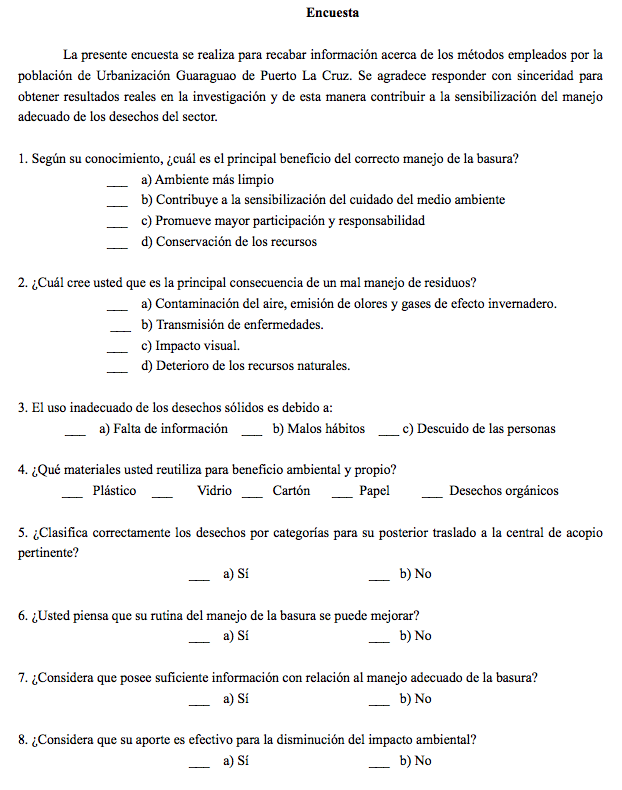
\includegraphics[width=12cm]{Media/Encuesta.png}
    \caption{Cuestionario de preguntas cerradas. \\[6pt] Autores: Diego Ortiz y Cynthia Cataldi}
    \label{fig:encuesta}
\end{figure}

\newpage

\section{Desarrollo de una campaña divulgativa sobre el manejo adecuado de los \\[6pt] desechos sólidos para la sensibilización del uso de las 3R de la ecología en \\[6pt] Urbanización Guaraguao de Puerto La Cruz}

párrafo párrafo párrafo párrafo párrafo párrafo párrafo párrafo párrafo párrafo párrafo párrafo párrafo párrafo párrafo párrafo párrafo párrafo 

\section{Seguimiento de las estrategias propuestas para el empleo de las 3R de la \\[6pt] ecología en Urbanización Guaraguao de Puerto La Cruz}

párrafo párrafo párrafo párrafo párrafo párrafo párrafo párrafo párrafo párrafo párrafo párrafo párrafo párrafo párrafo párrafo párrafo párrafo párrafo párrafo párrafo párrafo párrafo párrafo párrafo párrafo párrafo párrafo párrafo párrafo 

\newpage